\documentclass[a4paper,12pt]{extarticle}
\usepackage[utf8x]{inputenc}
\usepackage[T1,T2A]{fontenc}
\usepackage[russian]{babel}
\usepackage{hyperref}
\usepackage{indentfirst}
\usepackage{listings}
\usepackage{color}
\usepackage{xcolor}
\usepackage{here}
\usepackage{array}
\usepackage{multirow}
\usepackage{graphicx}
\usepackage{amsmath}

\hypersetup{
    colorlinks = false,
    linkbordercolor = {white}
}

\definecolor{string}{HTML}{B40000} % цвет строк в коде
\definecolor{comment}{HTML}{008000} % цвет комментариев в коде
\definecolor{keyword}{HTML}{1A00FF} % цвет ключевых слов в коде
\definecolor{morecomment}{HTML}{8000FF} % цвет include и других элементов в коде
\definecolor{сaptiontext}{HTML}{FFFFFF} % цвет текста заголовка в коде
\definecolor{сaptionbk}{HTML}{999999} % цвет фона заголовка в коде
\definecolor{bk}{HTML}{FFFFFF} % цвет фона в коде
\definecolor{frame}{HTML}{999999} % цвет рамки в коде
\definecolor{brackets}{HTML}{B40000} % цвет скобок в коде

\usepackage{caption}
\renewcommand{\lstlistingname}{Программа} % заголовок листингов кода

\bibliographystyle{ugost2008ls}

\usepackage{listings}
\lstset{ %
	extendedchars=\true,
	keepspaces=true,
	language=Python,						% choose the language of the code
	% Цвета
	keywordstyle=\color{keyword}\ttfamily\bfseries,
	%stringstyle=\color{string}\ttfamily,
	stringstyle=\ttfamily\color{red!50!brown},
	commentstyle=\color{comment}\ttfamily\itshape,
	morecomment=[l][\color{morecomment}]{\#},
	basicstyle=\footnotesize,		% the size of the fonts that are used for the code
	numbers=left,					% where to put the line-numbers
	numberstyle=\footnotesize,		% the size of the fonts that are used for the line-numbers
	stepnumber=1,					% the step between two line-numbers. If it is 1 each line will be numbered
	numbersep=5pt,					% how far the line-numbers are from the code
	backgroundcolor=\color{white},	% choose the background color. You must add \usepackage{color}
	showspaces=false				% show spaces adding particular underscores
	keywordstyle=color{blue}\bfseries, 
	showstringspaces=false,			% underline spaces within strings
	showtabs=false,					% show tabs within strings adding particular underscores
	frame=single,          		% adds a frame around the code
	tabsize=2,						% sets default tabsize to 2 spaces
	captionpos=t,					% sets the caption-position to top
	breaklines=true,				% sets automatic line breaking
	breakatwhitespace=false,		% sets if automatic breaks should only happen at whitespace
	escapeinside={\%*}{*)},			% if you want to add a comment within your code
	postbreak=\raisebox{0ex}[0ex][0ex]{\ensuremath{\color{red}\hookrightarrow\space}},
	texcl=true,
	inputpath=listings,                     % директория с листингами
}

\usepackage[left=2cm,right=2cm,
top=2cm,bottom=2cm,bindingoffset=0cm]{geometry}

%% Нумерация картинок по секциям
\usepackage{chngcntr}
\counterwithin{figure}{section}
\counterwithin{table}{section}

%%Точки нумерации заголовков
\usepackage{titlesec}
\titlelabel{\thetitle.\quad}
\usepackage[dotinlabels]{titletoc}

%% Оформления подписи рисунка
\addto\captionsrussian{\renewcommand{\figurename}{Рисунок}}
\captionsetup[figure]{labelsep = period}

%% Подпись таблицы
\DeclareCaptionFormat{hfillstart}{\hfill#1#2#3\par}
\captionsetup[table]{format=hfillstart,labelsep=newline,justification=centering,skip=-10pt,textfont=bf}

%% Путь к каталогу с рисунками
\graphicspath{{fig/}}

\begin{document}	% начало документа

% Титульная страница
%\begin{titlepage}	% начало титульной страницы

	\begin{center}		% выравнивание по центру

		Санкт-Петербургский Национально Исследовательский Университет\\
		информационных технологий, механики и оптики \\
		Кафедра систем управления и информатики\\[3cm]
		% название института, затем отступ 6см
		
		\huge \textbf{РЕФЕРАТ}\\[0.5cm]
		\large Электромеханические системы\\[0.1cm]
		\large Система автоматического управления квадракоптера Parrot ARDrone 2.0\\[2cm]

	\end{center}


	\begin{flushright} % выравнивание по правому краю
%		\begin{minipage}{0.5\textwidth} % врезка в половину ширины текста
%			\begin{flushleft} % выровнять её содержимое по левому краю

				\large Выполнили студенты группы P3335\\
				\large А.М. Зенкин\\[0.5cm]
				\large К.В. Карпов\\[0.5cm]
				
				\large Принял  к.т.н., доцент кафедры СУиР\\
				\sign[4cm]\large  М.С. Чежин\\
				\large Оценка: \sign\\
				«\underline{\hspace{0.7cm}}» \underline{\hspace{2cm}} \the\year г.

%			\end{flushleft}
%		\end{minipage}
	\end{flushright}
	
	\vfill % заполнить всё доступное ниже пространство

	\begin{center}
	\large Санкт-Петербург\\
	\large \the\year % вывести дату
	\end{center} % закончить выравнивание по центру

\thispagestyle{empty} % не нумеровать страницу
%\end{titlepage} % конец титульной страницы
\newpage


% Содержание
% Содержание
\renewcommand\contentsname{\centerline{Содержание}}
\tableofcontents
\thispagestyle{fancy}
\newpage




\section{Цель работы}
Изучение команд для получения информации о системе.Получить навыки работы с каталогами, папками и файлами в ОС Linux Ubuntu. 


\section{Задание 1.1 Средства просмотра системной информации}

\subsection{uname - консольная UNIX-утилита, выводящая информацию о системе.}

\begin{figure}[H]
	\begin{center}
		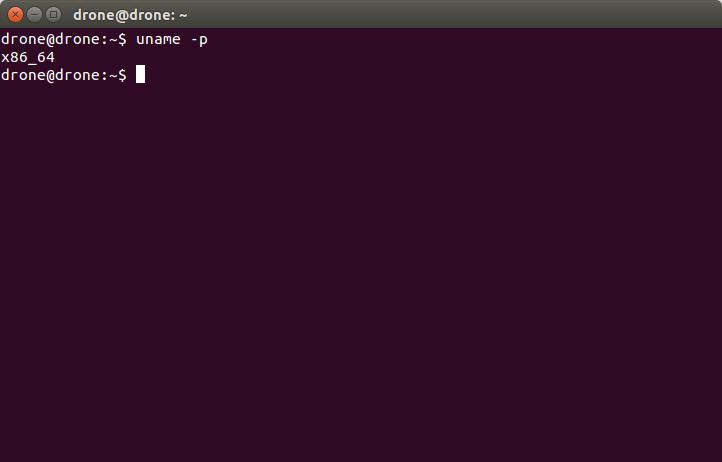
\includegraphics[scale=0.5]{type_of_processor}
		\caption{Тип процессора} 
		\label{pic:pic_1} % название для ссылок внутри кода
	\end{center}
\end{figure}

\newpage

\subsection{date — утилита Unix для работы с системными часами. Выводит текущую дату и время в различных форматах и позволяет устанавливать системное время.}

\begin{figure}[H]
	\begin{center}
		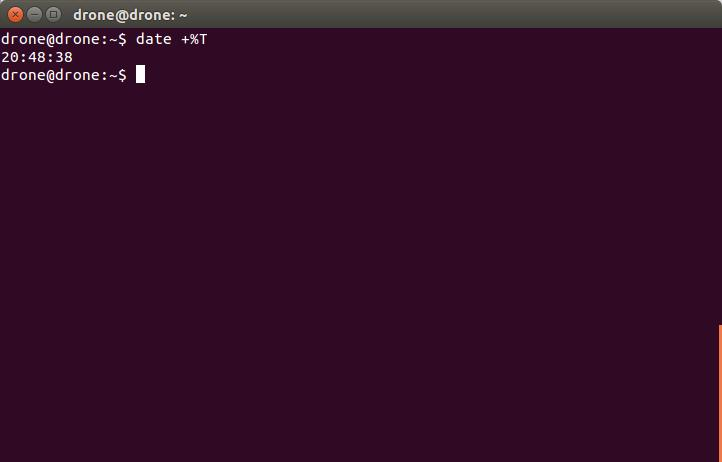
\includegraphics[scale=0.5]{time_1}
		\caption{Текущее время 1} 
		\label{pic:pic_2} % название для ссылок внутри кода
	\end{center}
\end{figure}

\begin{figure}[H]
	\begin{center}
		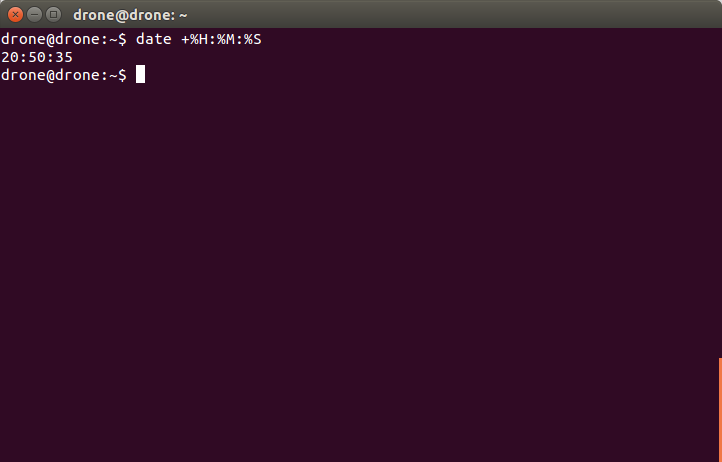
\includegraphics[scale=0.5]{time_2}
		\caption{Текущее время 2} 
		\label{pic:pic_3} % название для ссылок внутри кода
	\end{center}
\end{figure}

\newpage


\section{Задание 1.2 Команды для работы с каталогами, папками и файлами}

\subsection{Отображаем текущее положение (путь к директории, в которой мы сейчас находимся).}

\subsubsection{pwd}
Консольная утилита в UNIX-подобных системах, которая выводит полный путь от корневого каталога к текущему рабочему каталогу: в контексте которого (по умолчанию) будут исполняться вводимые команды.

\begin{figure}[H]
	\begin{center}
		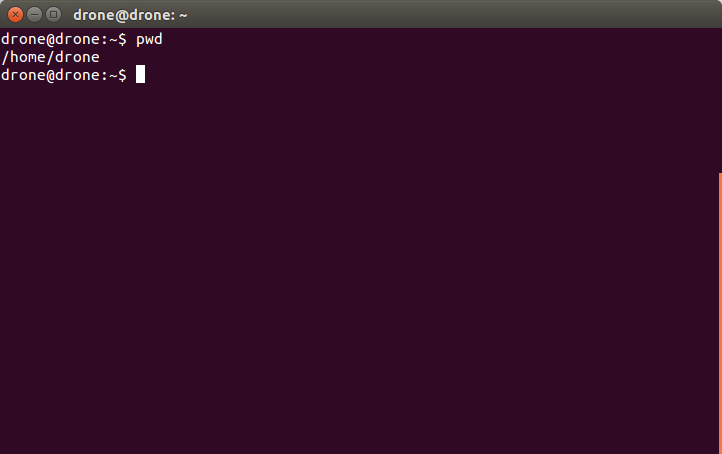
\includegraphics[scale=0.5]{1}
		\caption{} 
		\label{pic:pic_4} % название для ссылок внутри кода
	\end{center}
\end{figure}

\newpage

\subsection{Создали директорию 1. Подтвердили создание папки (вывели содержимое директории). Перешли в эту папку.}

\subsubsection{cd}
Команда cd позволяет перемещаться из одного каталога в другой.
\subsubsection{mkdir}
Команда для создания новых каталогов.
\subsubsection{ls}
Команда, которая печатает в стандартный вывод содержимое каталогов.

\begin{figure}[H]
	\begin{center}
		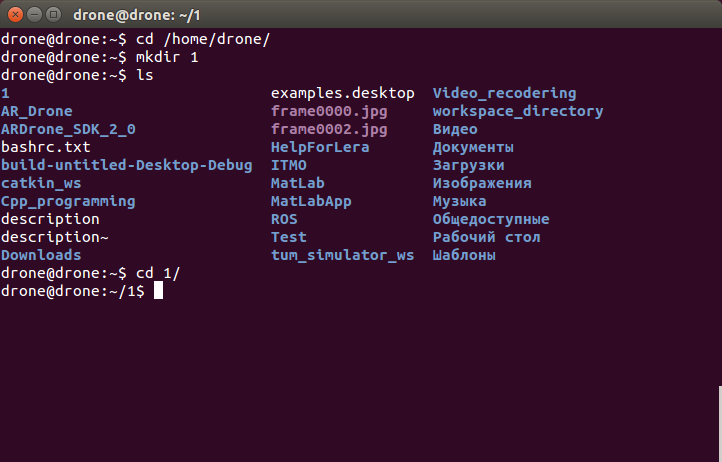
\includegraphics[scale=0.5]{2}
		\caption{} 
		\label{pic:pic_5} % название для ссылок внутри кода
	\end{center}
\end{figure}

\subsection{Создали одновременно в папке 1 папки Zenkin, Karpov. Подтвердили создание папки.}

\begin{figure}[H]
	\begin{center}
		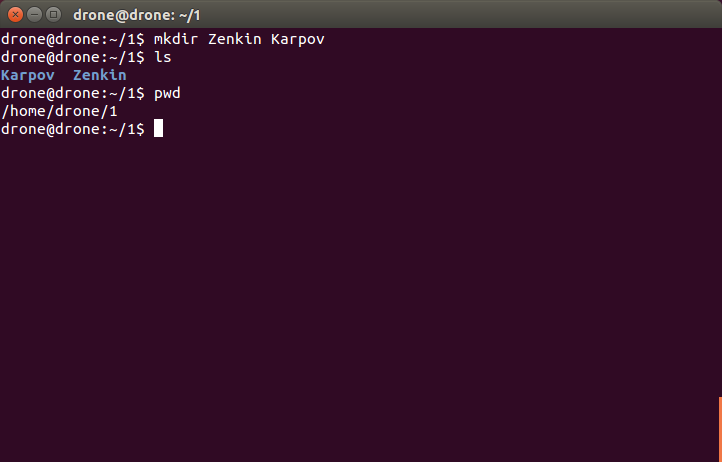
\includegraphics[scale=0.5]{3}
		\caption{} 
		\label{pic:pic_6} % название для ссылок внутри кода
	\end{center}
\end{figure}

\subsection{Не переходя в папку Zenkin создали папку ArtemiiKarpovKonstantin.  Подтвердить создание папки. }

\begin{figure}[H]
	\begin{center}
		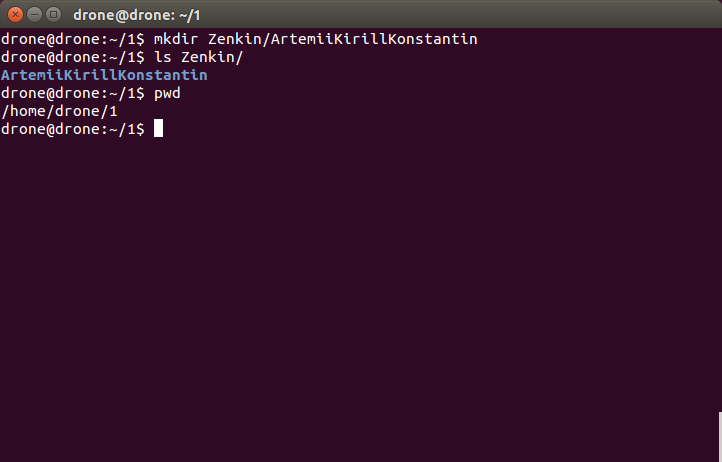
\includegraphics[scale=0.5]{4}
		\caption{} 
		\label{pic:pic_7} % название для ссылок внутри кода
	\end{center}
\end{figure}

\subsection{Перешли в папку ArtemiiKarpovKonstantin(используя относительный путь). Одновременно создали два файла Artemii и Kirill. Подтвердили создание файлов.}

\subsubsection{touch}
Команда Unix, предназначенная для установки времени последнего изменения файла или доступа в текущее время. Также используется для создания пустых файлов.

\begin{figure}[H]
	\begin{center}
		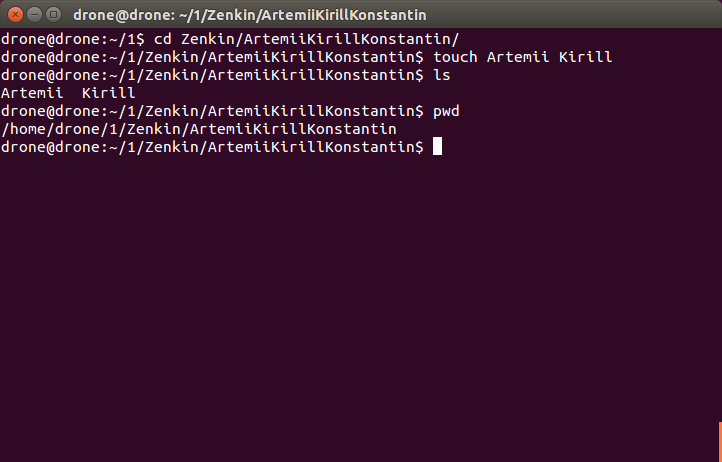
\includegraphics[scale=0.5]{5}
		\caption{} 
		\label{pic:pic_8} % название для ссылок внутри кода
	\end{center}
\end{figure}

\newpage

\subsection{Создали file4, не переходя в. Подтвердили создание файла.}

\begin{figure}[H]
	\begin{center}
		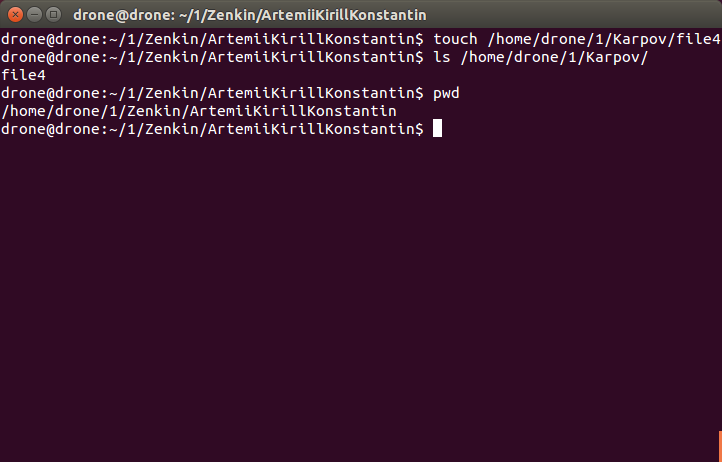
\includegraphics[scale=0.5]{6}
		\caption{} 
		\label{pic:pic_9} % название для ссылок внутри кода
	\end{center}
\end{figure}

\subsection{Скопировали папку ArtemiiKirillKonstantin в папку 1 со всем содержимым. Подтвердили.}

\subsubsection{cp}
Команда Unix в составе GNU Coreutils, предназначенная для копирования файлов из одного в другие каталоги (возможно, с другой файловой системой). Исходный файл остаётся неизменным, имя созданного файла может быть таким же, как у исходного, или изменится.

\begin{figure}[H]
	\begin{center}
		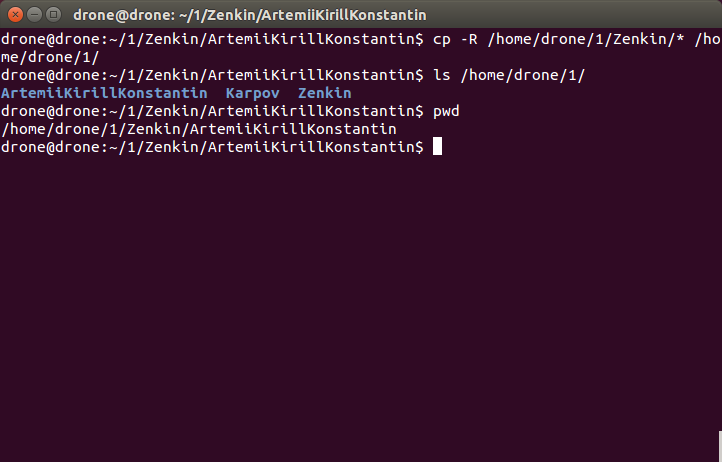
\includegraphics[scale=0.5]{7}
		\caption{} 
		\label{pic:pic_10} % название для ссылок внутри кода
	\end{center}
\end{figure}

\subsection{Из папки ArtemiiKirillKonstantin скопировали файл с именем, соответствующим фамилии Zenkin в папку Zenkin. Удалили папку ArtemiiKirillKonstantin со всем содержимым. Подтвердили.}

\subsubsection{rm}
Утилита в UNIX и UNIX-подобных системах, используемая для удаления файлов из файловой системы.

\begin{figure}[H]
	\begin{center}
		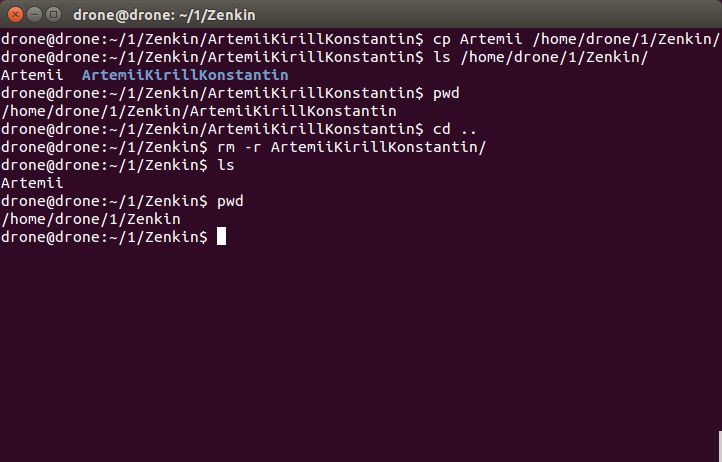
\includegraphics[scale=0.5]{8}
		\caption{} 
		\label{pic:pic_11} % название для ссылок внутри кода
	\end{center}
\end{figure}

\newpage

\subsection{Одновременно переименовали file4 в «Пустой» и переместили его в папку 1. Подтвердили.}

\subsubsection{mv}
Утилита в UNIX и UNIX-подобных системах, используется для перемещения или переименования файлов.

\begin{figure}[H]
	\begin{center}
		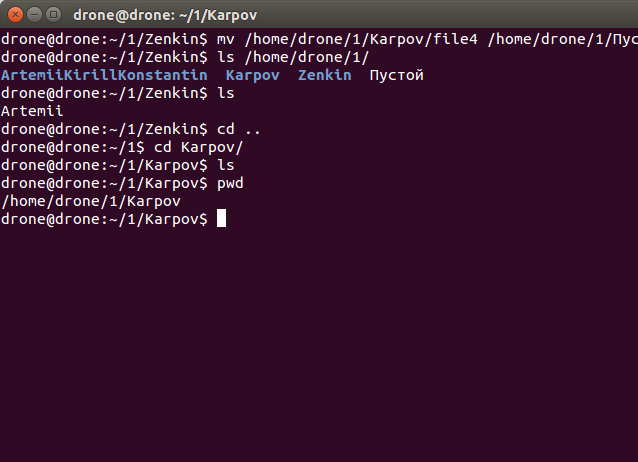
\includegraphics[scale=0.5]{9}
		\caption{} 
		\label{pic:pic_12} % название для ссылок внутри кода
	\end{center}
\end{figure}

\newpage

\subsection{Из папки ArtemiiKirillKonstantin переместили файлы с именами в Karpov. Подтвердили. Оставили в папке файл, соответствующий фамилии, другой файл удалили.  Подтвердили. Удалили пустую папку ArtemiiKirillKonstantin (используя команду для удаления пустой папки). Просмотрели содержимое папок 1, Zenkin, Karpov.}

\subsubsection{find}
Утилита поиска файлов по имени и другим свойствам, используемая в UNIX-подобных операционных системах.
\begin{figure}[H]
	\begin{center}
		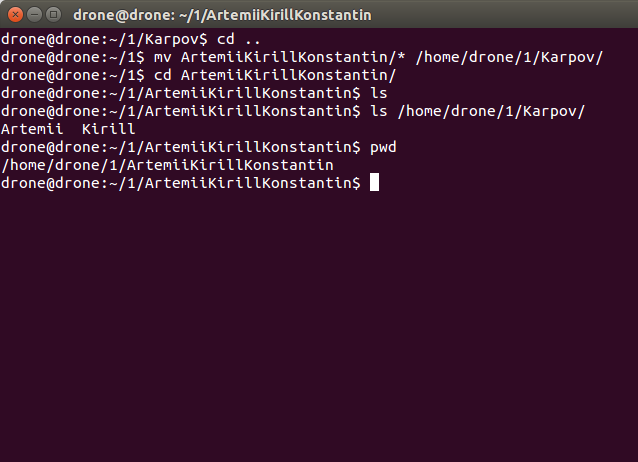
\includegraphics[scale=0.5]{10}
		\caption{} 
		\label{pic:pic_13} % название для ссылок внутри кода
	\end{center}
\end{figure}

\begin{figure}[H]
	\begin{center}
		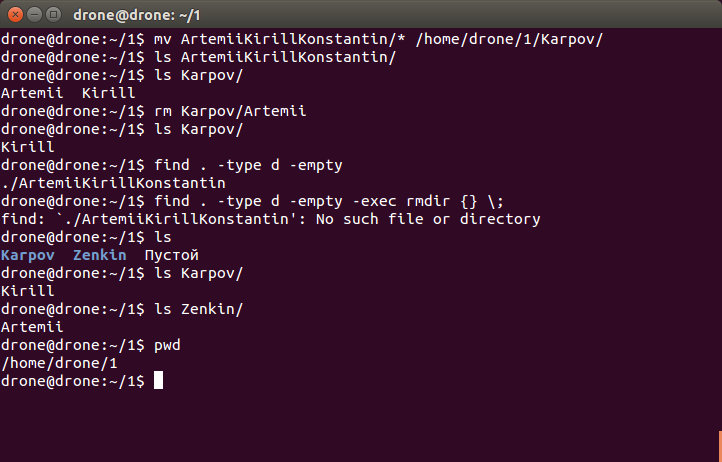
\includegraphics[scale=0.44]{11}
		\caption{} 
		\label{pic:pic_14} % название для ссылок внутри кода
	\end{center}
\end{figure}

\subsection{Перешли из текущей папки в папку 1, используя специальные символы. Создали текстовый документ file1 (запустив консольный текстовый редактор) и записали в него текст: «Все задания выполнили. Команды для работы с папками, файлами и каталогами выучили». Сохранили файл под названием finita. Сделали скрин текстового редактора с введенным текстом. Подтвердили наличие файла.}

\subsubsection{nano}
Консольный текстовый редактор для UNIX.
\begin{figure}[H]
	\begin{center}
		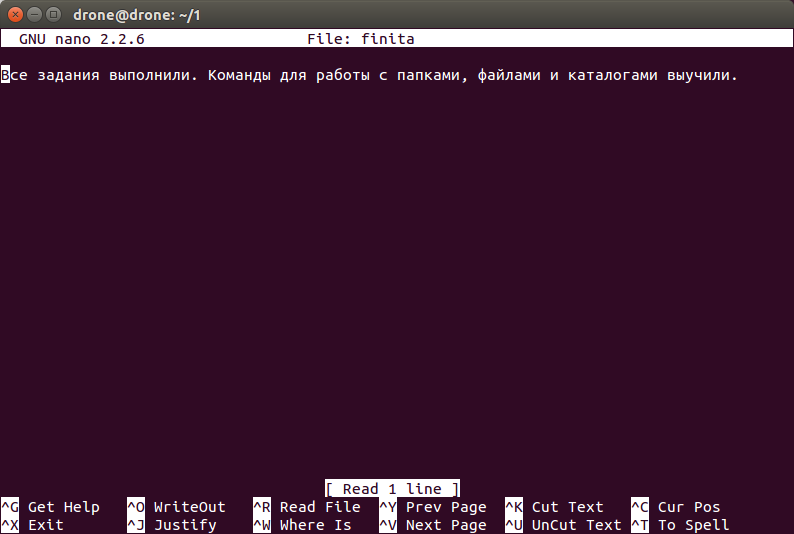
\includegraphics[scale=0.5]{12}
		\caption{} 
		\label{pic:pic_15} % название для ссылок внутри кода
	\end{center}
\end{figure} 

\begin{figure}[H]
	\begin{center}
		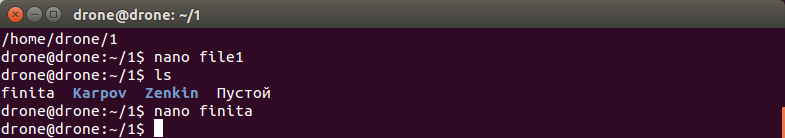
\includegraphics[scale=0.5]{13}
		\caption{} 
		\label{pic:pic_16} % название для ссылок внутри кода
	\end{center}
\end{figure}

\subsection{Вывели содержание файла finite в терминале.}

\subsubsection{cat}
утилита UNIX, выводящая последовательно указанные файлы (или устройства), таким образом, объединяя их в единый поток.

\begin{figure}[H]
	\begin{center}
		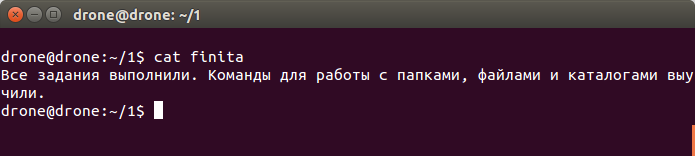
\includegraphics[scale=0.5]{14}
		\caption{} 
		\label{pic:pic_18} % название для ссылок внутри кода
	\end{center}
\end{figure}

\section{Вывод}
В данно лабораторной работе были изучены команды для получения информации о системе, а также навыки работы с каталогами, папками и файлами в ОС Linux Ubuntu. 
\end{document}
